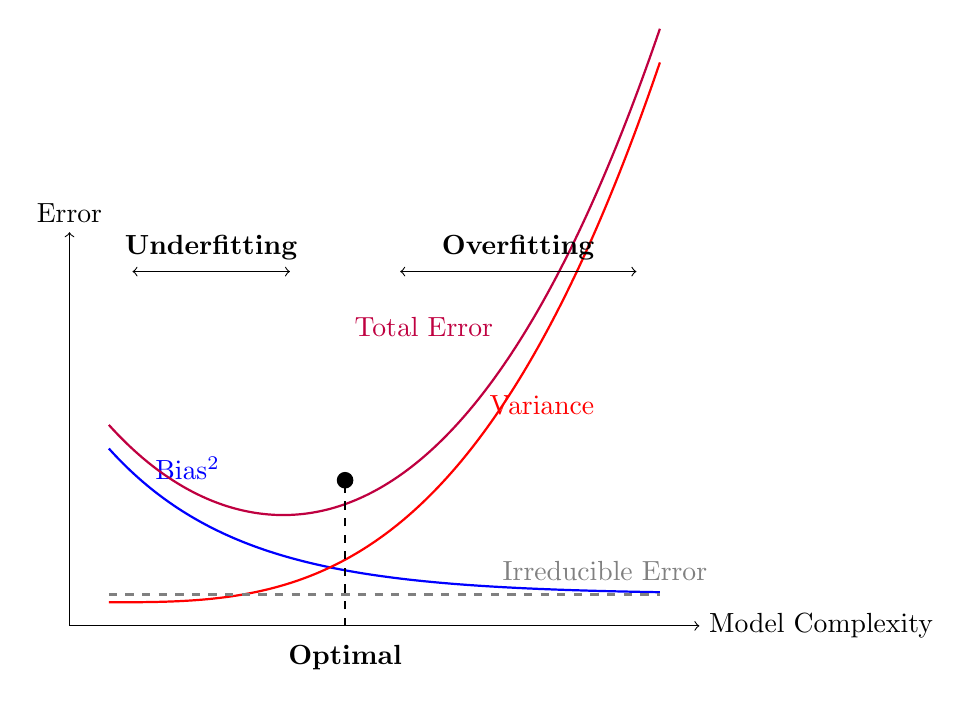
\begin{tikzpicture}[scale=1.0]
  \draw[->] (0,0) -- (8,0) node[right] {Model Complexity};
  \draw[->] (0,0) -- (0,5) node[above] {Error};
  
  % Bias curve (smoother decreasing)
  \draw[thick, blue, domain=0.5:7.5, samples=150] plot (\x, {2.5*exp(-0.6*\x) + 0.4});
  \node[blue] at (1.5, 2.0) {Bias$^2$};
  
  % Variance curve (smoother increasing)
  \draw[thick, red, domain=0.5:7.5, samples=150] plot (\x, {0.02*(\x-0.5)^3 + 0.3});
  \node[red] at (6, 2.8) {Variance};
  
  % Total error curve (smoother U-shape)
  \draw[thick, purple, domain=0.5:7.5, samples=150] plot (\x, {2.5*exp(-0.6*\x) + 0.02*(\x-0.5)^3 + 0.7});
  \node[purple] at (4.5, 3.8) {Total Error};
  
  % Irreducible error line
  \draw[thick, gray, dashed] (0.5, 0.4) -- (7.5, 0.4);
  \node[gray] at (6.8, 0.7) {Irreducible Error};
  
  % Optimal point - more prominent
  \coordinate (opt) at (3.5, 1.85);
  \draw[thick, black, dashed] (3.5, 0) -- (opt);
  \fill[black] (opt) circle (3pt);
  \node[black] at (3.5, -0.4) {\textbf{Optimal}};
  
  % Region labels with arrows
  \draw[<->] (0.8, 4.5) -- (2.8, 4.5);
  \node at (1.8, 4.8) {\textbf{Underfitting}};
  \draw[<->] (4.2, 4.5) -- (7.2, 4.5);
  \node at (5.7, 4.8) {\textbf{Overfitting}};
\end{tikzpicture}
